\documentclass{report}
\usepackage{graphicx}
\usepackage[hidelinks]{hyperref}
\usepackage{cite}
\begin{document}
\begin{titlepage}
    \begin{center}
        \vspace{1.0cm}
        
\includegraphics[scale=0.5]{Warwick}
        \vspace*{1cm}
  
        % Title
        \textbf{Using Ad Hoc Networking in Emergency Situations}
  
        \vspace{0.5cm}
        % Subtitle
        Spreading information in an emergency situation to help both people in danger and the emergency services
  
        \vspace{1.5cm}

        % What the project is about
        \textbf{Project Specification}
  
        \vspace{1.6cm}

        % Author name
        \textbf{Freddie Brown}\\
        \textbf{u1716717}


  
        \vspace{1.6cm}
        % Information about the institution
        Supervisor: Dr. Matthew Leeke\\
        Department of Computer Science\\
        University of Warwick\\
        2019-20
  
    \end{center}
\end{titlepage}


\chapter{Abstract}
\pagenumbering{roman}
\addcontentsline{toc}{chapter}{Abstract}

During a disaster, it is often very difficult to communicate using our devices. Whether this be because 
infrastructure has been damaged, or there is too much traffic over networks. This can mean people feel 
isolated and makes it difficult for the emergency services to know the situation on the ground. This 
project aims to help ease this by creating emergency Ad-Hoc networks during times of emergency. Using 
hardware already found in the devices people carry around with them day-to-day, information can be 
passed from person to person and can be sent to the emergency services or out over an internet connection. 
It allows survivors of these kinds of situations to maintain contact with the rest of the world.  
\\
\\
\textit{Keywords: Bluetooth, Ad Hoc, MANET, Emergency, Disaster}


% \chapter*{Acknowledgements}
% \addcontentsline{toc}{chapter}{Acknowledgements}
% Acknowledgements

\chapter{Abbreviations}
\addcontentsline{toc}{chapter}{Abbreviations}

\textbf{MANET} - Mobile Ad Hoc Network\\
\textbf{VM} - Virtual Machine\\
\textbf{BCS} - British Computing Society\\
\textbf{WSN} - Wireless Sensor Network\\
\textbf{AODV} - Ad-Hoc On-Demand Distance Vector\\
\textbf{DTN} - Delay Tolerant Network\\
\textbf{LSR} - Link-State Routing\\



\tableofcontents{}     

\chapter{Introduction}
\pagenumbering{arabic}



\section{Motivations}


\section{Project Aims}

\section{Stakeholders}


\chapter{Research}

\section{Different Implementations}
 

\section{Data Privacy}


\section{Routing}


\chapter{Ethical, Social, Legal and Professional Issues}

\section{Ethical Issues}

Ethical issues arise when there are competing objectives  where some have unclear negatives. An example of this 
is using data collected through using a product to target certain groups without their consent. 
A firm may make more money by doing this, but whether it is right to do so is something that 
should be considered. Fundamentally, stakeholders in the project should be protected and their 
data shouldn't be used against them. Data should be kept anonymous and protected somehow, through 
traditional encryption or other means. 

\section{Social Issues}

Social issues are those that may have an affect on the lives of many people. It could be problems which 
affect how they interact with other people or those relating to access to goods and services that others can 
but they can't. Currently, it is hard to see any issues of this nature relating to the project but this should 
be continually considered as the project moves forward.

\section{Legal Issues}

This project will deal with sending data about an individual to others and allowing them to hold and send this 
data to whomever they wish to send it to. There are legal issues as, without proper protections, this kind of 
data could be used against individuals that are in trouble, such as in a terror incident. 
\bigskip
\\
In this project, sensitive data will be dealt with appropriately, such as location data, so no one is privy to this 
information at any time if they shouldn't have access to it. As discussed above in Ethical Issues, this should be 
done by maintaining data privacy through encryption or other means.

\section{Professional Issues}

This project will adhere to the BCS Code of Conduct\cite{BCSCoP}. The aim is to produce a 
research project which can be trusted and respected and so adherence to all rules that are required 
is important. This means I will also follow the Research Code of Practice at the University of Warwick\cite{UniWarwickCOP}. 
This means all work I use to support my research will be referenced. 

\chapter{Project Requirements}

\section{Functional}

\textbf{FR1} - The system must use a widely used MAC layer protocol such as Bluetooth or WiFi.\\
$\newline$


\section{Non-Functional}

\textbf{NFR1} - The system must be fully documented and maintainable. This means that the project is easily extensible and can easily be implemented on other platforms.\\
$\newline$
\textbf{NFR2} - The system must be easy for a user to connect to and use. This is vital for the project as time is an important factor in an emergency situation and so 
the less time a user has to worry about how it works, the quicker they can use it to get help\\
$\newline$
\textbf{NFR3} - The system must be created so it can be applied to a large population of devices. This project works optimally if there are a large number of devices to connect 
so design choices should consider the need for this project to work at a large scale.\\
$\newline$
\textbf{NFR4} - The system must be able to be used by different types of devices such as Phones, Tablets and PCs. Much like \textbf{NFR3}, this project should be designed so it can 
be easily transported onto other devices so that they can also participate.\\
$\newline$


\section{Constraints}

This project will be constrained by the number of devices which it can be tested on and the type of devices which can be used. Having access 
to lots of devices can be very expensive. This project will use Raspberry Pi's to demonstrate the application of the research but these cost 
money and it won't be able to replicate the scale at which an emergency situation may be.
\bigskip\\
A further constraint will be the types of devices. The research will focus on applications in a heterogenous network of devices but it is 
likely this will only be demonstrated on a homogenous network as more popular devices (e.g iOS and Android\cite{mobileOS}), which this type of system would be employed on in the 
real world, don't allow root access and are restrictive about what can be run on devices. This makes them difficult to develop for on this project, but are platforms which 
this would need be implemented on in the real world.

\chapter{Project Management}

\section{Project Timeline}
\begin{figure}
    \centering
    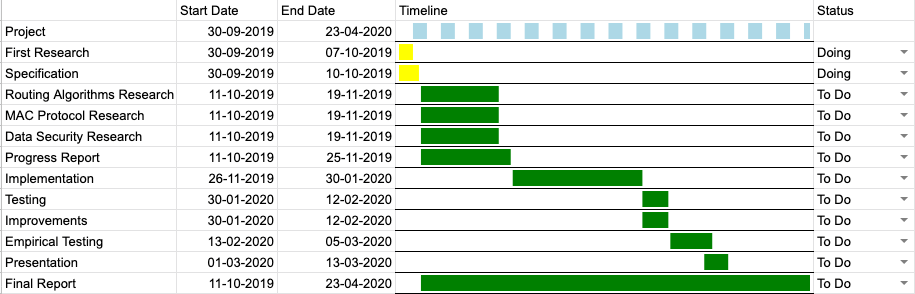
\includegraphics[scale=0.35]{ProjectTimeline}
    \caption{Project Timeline}
    \label{fig:project-timeline}
\end{figure}
\bigskip

As can be seen in fig.\ref{fig:project-timeline}, it shows the predicted project timeline in a Gantt chart as well as displaying the dates between 
which each task will take place. Looking at the timeline, ample time has been left for research for the different aspects of the 
project (about a month). During this time, the second project deliverable can also be written. After this, a large block of time 
has been left for the implementation of the project, about 2 months. After this, a period of product testing and iteration has been 
scheduled so that bugs and improvements can be made so it performs better. After this, further testing will take place where results 
of the performance of the project can be collected so they can be presented in the final report and presentation. 

\section{Project Tools}

This project will use C++ for programming. This has been chosen because it is a low level programming language 
so the code will be easier to optimise for increased performance. A library which will be used to interface with Bluetooth with is BlueZ\cite{bluez}. This will 
provide a good api to interface with Bluetooth with on Linux machines.
\bigskip\\
In terms of hardware, the project is going to be written for Linux-based devices such as the Raspberry Pi which have 
Bluetooth. This is a pretty basic requirement for the hardware as Bluetooth is standard on a lot of devices. Having 
very few requirements lowers barrier to entry to use the project and makes it easier to see how it could 
be used on a variety of devices. 
\bigskip\\
A variety of other tools will be used for other aspects of the project. Trello will be used to keep track of tasks that 
need to be done. This is a simple and clear way to see what it left to do and allows deadlines to be built into tasks. It 
also fits in with an Agile development methodology, which is preferable. On top of this, Git and Github will be used as the version 
control system to store code. It makes it easier to access project resources from multiple locations and provides a good back 
up if something went wrong and all physical devices which hold the project, were to break for some unforeseen reason. 

\section{Risk Management}

In this project, there aren't too many major risks that could have an effect on its performance. One risk, which was discussed 
above, is losing all physical machines which hold the project. This can be mitigated by storing any code and reports on Github, 
as well as maintaining a local copy on a hard drive. This provides extra layers of assurance that the project won't be lost. 
\bigskip\\
Another risk is that persons who work on the project fall ill or are unable to do work. This can be mitigated by keeping in 
contact with DCS and discussing any factors that could lead to a delay in the projects completion because of this reason.
\bigskip\\
Furthermore, there is always a risk that something might take longer than it is planned for to complete. This could be because hardware 
access has been delayed or there are extra technical difficulties that weren't foreseen during the planning of the project. Because of this, 
generous allowances have been made for each task in the project. If something finishes earlier than planned, other tasks can use this time. 
Also, if a task is running late, subsequent tasks have extra time built in to accommodate for any delays.

\chapter{Testing}

Testing in this project will be used to verify the functionality of the project while changes are made as 
well as being able to verify that requirements have been fulfilled. The project will use a couple of different 
technologies to accomplish this. For unit testing an established C++-specific framework will be used, such 
as CppUnit.
For integration testing, TravisCI will be used. Once more, its a robust service and it has very good integration with Github and 
is very customisable. 

\section{Unit Testing}

With unit testing, tests will be written for each feature that is created. These will be lined up with the requirements so that 
it is easy to see that they are being fulfilled. For writing unit tests, Agile development methodologies will be adhered to by 
writing the tests before writing the feature. Unit testing and its benefits are further discussed in \cite{PressmanUnitIntegration, SommervilleTDD}. 
In these, they discuss the benefits of Test Driven Development and how unit testing works and is beneficial to a project. 

\section{Integration Testing}

By using TravisCI, larger tests can be written which incorporated more of the project. This can be run on a clean VM which 
means there is nothing external to the project which could influence its testing. This enables more rigorous testing. This 
approach to testing the system is discussed in \cite{PressmanUnitIntegration}.

\section{Success Management}

The way success of the project can be measured is if the project can transmit packets across a group of devices with to a 
target device. This would simulate a device in a disaster scenario which is either the emergency services or an internet 
connected device. This will be tested on a number of topologies and in different environments to test performance when taking 
in lots of different physical and real world factors.


\chapter{Conclusion}



\bibliography{ref}{}
\bibliographystyle{IEEEtran}

\end{document}
